\documentclass{ximera}

%\usepackage{todonotes}

\newcommand{\todo}{}

\usepackage{esint} % for \oiint
\ifxake%%https://math.meta.stackexchange.com/questions/9973/how-do-you-render-a-closed-surface-double-integral
\renewcommand{\oiint}{{\large\bigcirc}\kern-1.56em\iint}
\fi


\graphicspath{
  {./}
  {ximeraTutorial/}
  {basicPhilosophy/}
  {functionsOfSeveralVariables/}
  {normalVectors/}
  {lagrangeMultipliers/}
  {vectorFields/}
  {greensTheorem/}
  {shapeOfThingsToCome/}
  {dotProducts/}
  {partialDerivativesAndTheGradientVector/}
  {../productAndQuotientRules/exercises/}
  {../normalVectors/exercisesParametricPlots/}
  {../continuityOfFunctionsOfSeveralVariables/exercises/}
  {../partialDerivativesAndTheGradientVector/exercises/}
  {../directionalDerivativeAndChainRule/exercises/}
  {../commonCoordinates/exercisesCylindricalCoordinates/}
  {../commonCoordinates/exercisesSphericalCoordinates/}
  {../greensTheorem/exercisesCurlAndLineIntegrals/}
  {../greensTheorem/exercisesDivergenceAndLineIntegrals/}
  {../shapeOfThingsToCome/exercisesDivergenceTheorem/}
  {../greensTheorem/}
  {../shapeOfThingsToCome/}
  {../separableDifferentialEquations/exercises/}
  {vectorFields/}
}

\newcommand{\mooculus}{\textsf{\textbf{MOOC}\textnormal{\textsf{ULUS}}}}

\usepackage{tkz-euclide}
\usepackage{tikz}
\usepackage{tikz-cd}
\usetikzlibrary{arrows}
\tikzset{>=stealth,commutative diagrams/.cd,
  arrow style=tikz,diagrams={>=stealth}} %% cool arrow head
\tikzset{shorten <>/.style={ shorten >=#1, shorten <=#1 } } %% allows shorter vectors

\usetikzlibrary{backgrounds} %% for boxes around graphs
\usetikzlibrary{shapes,positioning}  %% Clouds and stars
\usetikzlibrary{matrix} %% for matrix
\usepgfplotslibrary{polar} %% for polar plots
\usepgfplotslibrary{fillbetween} %% to shade area between curves in TikZ
%\usetkzobj{all}
\usepackage[makeroom]{cancel} %% for strike outs
%\usepackage{mathtools} %% for pretty underbrace % Breaks Ximera
%\usepackage{multicol}
\usepackage{pgffor} %% required for integral for loops



%% http://tex.stackexchange.com/questions/66490/drawing-a-tikz-arc-specifying-the-center
%% Draws beach ball
\tikzset{pics/carc/.style args={#1:#2:#3}{code={\draw[pic actions] (#1:#3) arc(#1:#2:#3);}}}



\usepackage{array}
\setlength{\extrarowheight}{+.1cm}
\newdimen\digitwidth
\settowidth\digitwidth{9}
\def\divrule#1#2{
\noalign{\moveright#1\digitwidth
\vbox{\hrule width#2\digitwidth}}}




% \newcommand{\RR}{\mathbb R}
% \newcommand{\R}{\mathbb R}
% \newcommand{\N}{\mathbb N}
% \newcommand{\Z}{\mathbb Z}

\newcommand{\sagemath}{\textsf{SageMath}}


%\renewcommand{\d}{\,d\!}
%\renewcommand{\d}{\mathop{}\!d}
%\newcommand{\dd}[2][]{\frac{\d #1}{\d #2}}
%\newcommand{\pp}[2][]{\frac{\partial #1}{\partial #2}}
% \renewcommand{\l}{\ell}
%\newcommand{\ddx}{\frac{d}{\d x}}

% \newcommand{\zeroOverZero}{\ensuremath{\boldsymbol{\tfrac{0}{0}}}}
%\newcommand{\inftyOverInfty}{\ensuremath{\boldsymbol{\tfrac{\infty}{\infty}}}}
%\newcommand{\zeroOverInfty}{\ensuremath{\boldsymbol{\tfrac{0}{\infty}}}}
%\newcommand{\zeroTimesInfty}{\ensuremath{\small\boldsymbol{0\cdot \infty}}}
%\newcommand{\inftyMinusInfty}{\ensuremath{\small\boldsymbol{\infty - \infty}}}
%\newcommand{\oneToInfty}{\ensuremath{\boldsymbol{1^\infty}}}
%\newcommand{\zeroToZero}{\ensuremath{\boldsymbol{0^0}}}
%\newcommand{\inftyToZero}{\ensuremath{\boldsymbol{\infty^0}}}



% \newcommand{\numOverZero}{\ensuremath{\boldsymbol{\tfrac{\#}{0}}}}
% \newcommand{\dfn}{\textbf}
% \newcommand{\unit}{\,\mathrm}
% \newcommand{\unit}{\mathop{}\!\mathrm}
% \newcommand{\eval}[1]{\bigg[ #1 \bigg]}
% \newcommand{\seq}[1]{\left( #1 \right)}
% \renewcommand{\epsilon}{\varepsilon}
% \renewcommand{\phi}{\varphi}


% \renewcommand{\iff}{\Leftrightarrow}

% \DeclareMathOperator{\arccot}{arccot}
% \DeclareMathOperator{\arcsec}{arcsec}
% \DeclareMathOperator{\arccsc}{arccsc}
% \DeclareMathOperator{\si}{Si}
% \DeclareMathOperator{\scal}{scal}
% \DeclareMathOperator{\sign}{sign}


%% \newcommand{\tightoverset}[2]{% for arrow vec
%%   \mathop{#2}\limits^{\vbox to -.5ex{\kern-0.75ex\hbox{$#1$}\vss}}}
% \newcommand{\arrowvec}[1]{{\overset{\rightharpoonup}{#1}}}
% \renewcommand{\vec}[1]{\arrowvec{\mathbf{#1}}}
% \renewcommand{\vec}[1]{{\overset{\boldsymbol{\rightharpoonup}}{\mathbf{#1}}}}

% \newcommand{\point}[1]{\left(#1\right)} %this allows \vector{ to be changed to \vector{ with a quick find and replace
% \newcommand{\pt}[1]{\mathbf{#1}} %this allows \vec{ to be changed to \vec{ with a quick find and replace
% \newcommand{\Lim}[2]{\lim_{\point{#1} \to \point{#2}}} %Bart, I changed this to point since I want to use it.  It runs through both of the exercise and exerciseE files in limits section, which is why it was in each document to start with.

% \DeclareMathOperator{\proj}{\mathbf{proj}}
% \newcommand{\veci}{{\boldsymbol{\hat{\imath}}}}
% \newcommand{\vecj}{{\boldsymbol{\hat{\jmath}}}}
% \newcommand{\veck}{{\boldsymbol{\hat{k}}}}
% \newcommand{\vecl}{\vec{\boldsymbol{\l}}}
% \newcommand{\uvec}[1]{\mathbf{\hat{#1}}}
% \newcommand{\utan}{\mathbf{\hat{t}}}
% \newcommand{\unormal}{\mathbf{\hat{n}}}
% \newcommand{\ubinormal}{\mathbf{\hat{b}}}

% \newcommand{\dotp}{\bullet}
% \newcommand{\cross}{\boldsymbol\times}
% \newcommand{\grad}{\boldsymbol\nabla}
% \newcommand{\divergence}{\grad\dotp}
% \newcommand{\curl}{\grad\cross}
%\DeclareMathOperator{\divergence}{divergence}
%\DeclareMathOperator{\curl}[1]{\grad\cross #1}
% \newcommand{\lto}{\mathop{\longrightarrow\,}\limits}

% \renewcommand{\bar}{\overline}

\colorlet{textColor}{black}
\colorlet{background}{white}
\colorlet{penColor}{blue!50!black} % Color of a curve in a plot
\colorlet{penColor2}{red!50!black}% Color of a curve in a plot
\colorlet{penColor3}{red!50!blue} % Color of a curve in a plot
\colorlet{penColor4}{green!50!black} % Color of a curve in a plot
\colorlet{penColor5}{orange!80!black} % Color of a curve in a plot
\colorlet{penColor6}{yellow!70!black} % Color of a curve in a plot
\colorlet{fill1}{penColor!20} % Color of fill in a plot
\colorlet{fill2}{penColor2!20} % Color of fill in a plot
\colorlet{fillp}{fill1} % Color of positive area
\colorlet{filln}{penColor2!20} % Color of negative area
\colorlet{fill3}{penColor3!20} % Fill
\colorlet{fill4}{penColor4!20} % Fill
\colorlet{fill5}{penColor5!20} % Fill
\colorlet{gridColor}{gray!50} % Color of grid in a plot

\newcommand{\surfaceColor}{violet}
\newcommand{\surfaceColorTwo}{redyellow}
\newcommand{\sliceColor}{greenyellow}




\pgfmathdeclarefunction{gauss}{2}{% gives gaussian
  \pgfmathparse{1/(#2*sqrt(2*pi))*exp(-((x-#1)^2)/(2*#2^2))}%
}


%%%%%%%%%%%%%
%% Vectors
%%%%%%%%%%%%%

%% Simple horiz vectors
\renewcommand{\vector}[1]{\left\langle #1\right\rangle}


%% %% Complex Horiz Vectors with angle brackets
%% \makeatletter
%% \renewcommand{\vector}[2][ , ]{\left\langle%
%%   \def\nextitem{\def\nextitem{#1}}%
%%   \@for \el:=#2\do{\nextitem\el}\right\rangle%
%% }
%% \makeatother

%% %% Vertical Vectors
%% \def\vector#1{\begin{bmatrix}\vecListA#1,,\end{bmatrix}}
%% \def\vecListA#1,{\if,#1,\else #1\cr \expandafter \vecListA \fi}

%%%%%%%%%%%%%
%% End of vectors
%%%%%%%%%%%%%

%\newcommand{\fullwidth}{}
%\newcommand{\normalwidth}{}



%% makes a snazzy t-chart for evaluating functions
%\newenvironment{tchart}{\rowcolors{2}{}{background!90!textColor}\array}{\endarray}

%%This is to help with formatting on future title pages.
\newenvironment{sectionOutcomes}{}{}



%% Flowchart stuff
%\tikzstyle{startstop} = [rectangle, rounded corners, minimum width=3cm, minimum height=1cm,text centered, draw=black]
%\tikzstyle{question} = [rectangle, minimum width=3cm, minimum height=1cm, text centered, draw=black]
%\tikzstyle{decision} = [trapezium, trapezium left angle=70, trapezium right angle=110, minimum width=3cm, minimum height=1cm, text centered, draw=black]
%\tikzstyle{question} = [rectangle, rounded corners, minimum width=3cm, minimum height=1cm,text centered, draw=black]
%\tikzstyle{process} = [rectangle, minimum width=3cm, minimum height=1cm, text centered, draw=black]
%\tikzstyle{decision} = [trapezium, trapezium left angle=70, trapezium right angle=110, minimum width=3cm, minimum height=1cm, text centered, draw=black]



\author{Lee Wayand}

\begin{document}
\begin{exercise}





\[
H(k) = 
\begin{cases}
  -(k+4)(k-2)   & \text{ on } [-5, 2)   \\
  6              & \text{ if } k = 2 \\
  (k-2)(k-7)      & \text{ on } (2, 8]  
\end{cases}
\]






Graph of $y = H(k)$.



\begin{image}
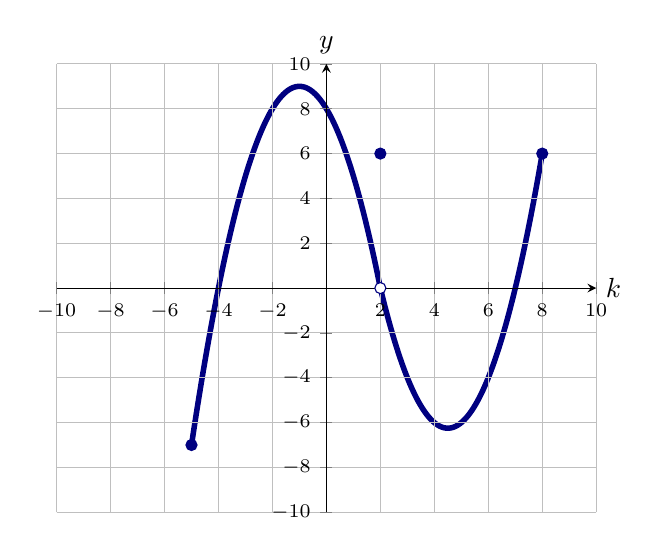
\begin{tikzpicture} 
  \begin{axis}[
            domain=-10:10, ymax=10, xmax=10, ymin=-10, xmin=-10,
            axis lines =center, xlabel=$k$, ylabel=$y$, grid = major,
            ytick={-10,-8,-6,-4,-2,2,4,6,8,10},
            xtick={-10,-8,-6,-4,-2,2,4,6,8,10},
            ticklabel style={font=\scriptsize},
            every axis y label/.style={at=(current axis.above origin),anchor=south},
            every axis x label/.style={at=(current axis.right of origin),anchor=west},
            axis on top
          ]
          
          \addplot [line width=2, penColor, smooth,samples=100,domain=(-5:2)] {-(x+4)*(x-2)};
       	  \addplot [line width=2, penColor, smooth,samples=100,domain=(2:8)] {(x-2)*(x-7)};
       		%\addplot [line width=2, penColor, smooth,samples=100,domain=(4:8)] {3*x-16};




			\addplot[color=penColor,fill=penColor,only marks,mark=*] coordinates{(-5,-7)};

			\addplot[color=penColor,fill=penColor,only marks,mark=*] coordinates{(2,6)};
			\addplot[color=penColor,fill=white,only marks,mark=*] coordinates{(2,0)};

			\addplot[color=penColor,fill=penColor,only marks,mark=*] coordinates{(8,6)};
			%\addplot[color=penColor,fill=white,only marks,mark=*] coordinates{(4,-4)};

			%\addplot[color=penColor,fill=white,only marks,mark=*] coordinates{(8,8)};

  \end{axis}
\end{tikzpicture}
\end{image}







\begin{question} Domain


The domain is given in the definition of the function.

\[
\left[ \answer{-5}, \answer{2} \right) \cup \left\{ \answer{2} \right\} \cup \left(  \answer{2}, \answer{8} \right] = \left[ \answer{-5}, \answer{8} \right]
\]


\end{question}







\begin{question} Continuity


The two pieces in the definition of $H(k)$ are quadratic functions.  These are continuous functions.  Therefore, the only candidate for discontinuity or singularity is $x = 2$.

The graph suggests that $x = 2$ is a discontinuity. We will show this is true. \\

Let $d = 1$. \\

For any small $\frac{1}{100} > \epsilon > 0$, the interval $(2 - \epsilon, 2)$ always contains the number $2 - \frac{\epsilon}{2}$.  


\[
H\left( 2 - \frac{\epsilon}{2} \right) = H\left( \frac{4 - \epsilon}{2} \right) = -\left( \frac{4 - \epsilon}{2} + 4 \right) \left(  \frac{4 - \epsilon}{2} - 2 \right)
\]

\[
= -\left( \frac{12 - \epsilon}{2} \right) \left(  \frac{- \epsilon}{2} \right) = \left( \frac{12 - \epsilon}{2} \right) \left(  \frac{\epsilon}{2} \right)
\]


Since, $\frac{1}{100} > \epsilon > 0$, $\frac{12 - \epsilon}{2} < 12$ and $\frac{\epsilon}{2} < \frac{1}{200}$


Therefore, 

\[
H\left( 2 - \frac{\epsilon}{2} \right) < \frac{12}{200} 
\]



On the interval, $(2 - \epsilon, 2)$, $H$ always has a value less than $\frac{12}{200}$.  Its distance from $H(2) = 6$ is greater than $d = 1$.



Perhaps the other side of $2$ would have been easier. \\

On the interval $(2, 2 + \epsilon)$, the second piece of $H$ is negative, which is more than $1$ away from $H(2) = 6$. \\


Every small open interval around $2$ contains a domain number where the value of $H$ is more than $1$ away from $H(2)$. \\


$x = 2$ is a discontinuity.



\end{question}





\begin{question} Zeros


The defininng pieces of $H$ have two zeros each.  The graph suggests that $x=2$ would be a zero for each quadratic piece, however, $H$ has moved this one value away from $0$.  That leaves two zeros for $H$.


\begin{explanation}



The left piece is a quadratic, which we have in factored form, $-(k+4)(k-2)$.  The zeros are $-4$ and $2$.  $H$ has redefined $H(2)$ to be $6$. \\


The right piece is a quadratic, which we have in factored form, $(k-2)(k-7)$.  The zeros are $2$ and $7$.  $H$ has redefined $H(2)$ to be $6$. \\


The zeros of $H$ are $\{ -4, 7 \}$.


\end{explanation}


\end{question}





\begin{question} End-Behavior



End-behavior is explicitly for unbounded domains.  Therefore, there is no end-behavior for $H$.


\end{question}






\begin{question} Behavior



From the graph, we can see that $H$ increases, then decreases, and then increases.  We want algebraic and functional reasoning. $iRoC_H(k)$ will give us behavior information.   \\


Avoiding the discontinuity, we have

\[
iRoC_H(k) = 
\begin{cases}
  \answer{-2k - 2}   & \text{ on } [-5, 2)   \\
  \answer{2k - 9}     & \text{ on } (2, 8]  
\end{cases}
\]



$-2k - 2$ gives us the critical number $\answer{-1}$. \\


$2k - 9$ gives us the critical number $\answer{\frac{9}{2}}$. \\





\begin{itemize}
\item $-2k - 2 \wordChoice{\choice{<} [correct]\choice{>}}  0$ on  $[-5, -1)$ where $H$ is increasing.
\item $-2k - 2 \wordChoice{\choice[correct]{<} \choice{>}}  0$ on  $(-1, 2)$ where $H$ is decreasing.
\item $2k - 9 \wordChoice{\choice[correct]{<} \choice{>}}  0$ on  $\left( 2, \frac{9}{2} \right)$ where $H$ is decreasing.
\item $2k - 9 \wordChoice{\choice{<} [correct]\choice{>}}  0$ on  $\left( \frac{9}{2}, 8 \right]$ where $H$ is increasing.
\end{itemize}







\begin{warning}


$H$ decreases on $[-1, 2)$ and on $\left( \frac{9}{2}, 8 \right]$, however, $H$ does not decrease on their union $[-1, 2) \cup \left( \frac{9}{2}, 8 \right]$.



We can show this algebraically, by providing a counterexample to the definition of decreasing. Select two domain numbers $a < b$, yet $f(a) < f(b)$.  Our two numbers will be $\frac{7}{4} < \frac{15}{2}$.


\begin{align*}
H\left( \frac{7}{4} \right) & = -\left( \frac{7}{4} + 4 \right) \left( \frac{7}{4} - 2 \right) \\
& = -\left( \frac{23}{4} \right) \left( -\frac{1}{4} \right) \\
& = \frac{23}{16}  
\end{align*}


\begin{align*}
H\left( \frac{15}{2} \right) & = \left( \frac{15}{2} - 2 \right) \left( \frac{15}{2} - 7 \right) \\
& = \left( \frac{11}{2} \right) \left( \frac{1}{2} \right) \\
& = \frac{11}{4}  
\end{align*}


\[
\frac{23}{16}  < \frac{32}{16} = 2 = \frac{8}{4} < \frac{11}{4} 
\]

\end{warning}


We now have a counterexample to the statement that $H$ is decreasing on the set $[-1, 2) \cup \left( \frac{9}{2}, 8 \right]$.





\end{question}








\end{exercise}
\end{document}